\section{Particle spectra and yields}
\label{secks:spectra}
\subsection{Charged-particle spectra}
\label{subsecks:transspectra}
Transverse momentum spectra of charged particles were measured by all three experiments exploiting the first collected data sample. They are presented as the dependence of the (inclusive) invariant cross section on the transverse momentum ($p_{\rm T}$), and finally in the form normalized to pp measurement at the same nucleon--nucleon energy. For the latter representation, the nuclear modification factor is defined as
\be
R_{\rm AA}(p_{\rm T}) = \frac{{\rm d}N_{\rm ch}^{\rm AA}(p_{\rm T})/{\rm d}p_{\rm T}}{\langle N_{\rm coll} \rangle \,{\rm d}N_{\rm ch}^{\rm pp}(p_{\rm T})/{\rm d}p_{\rm T}} ,
\label{eqks:RAA}
\ee
where on the right hand side the superscripts AA and pp refer to the values obtained in heavy-ion and pp measurements, respectively. If a collision of two nuclei behaved as a simple superposition of $N_{\rm coll}$ nucleon--nucleon collisions, the nuclear modification factor would be $R_{\rm AA} = 1$. Such a scaling with the number of binary collision $N_{\rm coll}$ is a natural expectation for hard processes, in case that nucleons act independently and their interactions are not influenced by the rest of the nuclei. This is observed for electro-weak bosons, since they practically do not interact with the surrounding medium, see Sec.~\ref{sect:pas:ew}. A deviation of $R_{\rm AA}$ from unity for hard processes signals a nuclear effect. However, for soft processes, such as particle production at $p_{\rm T}$ below a few GeV, the scaling from pp to AA is governed by $N_{\rm part}$ rather than by $N_{\rm coll}$, leading naturally to an $R_{\rm AA}$ below unity in that $p_{\rm T}$ region, especially for central events.

The $p_{\rm T}$ spectrum for charged particles in LHC heavy-ion collisions was expected to be suppressed at high $p_{\rm T}$ with respect to pp interactions. The fact that $R_{\rm AA}$ is significantly below unity at $p_{\rm T}$ above a few GeV was well established for central collisions at RHIC, and attributed to the jet quenching --- an energy loss of hard partons in their interactions with the surrounding high-density nuclear matter. As the high-$p_{\rm T}$ particles are supposed to be produced in the fragmentation of such hard partons, the shift to lower $p_{\rm T}$  by parton-energy loss decreases the particle production, reflecting the amount of energy loss, and thus the density of nuclear matter created in the collision. However, the value of $R_{\rm AA}$ is also dependent on the steepness of the parton $p_{\rm T}$ spectrum (for fixed parton energy loss, a harder parton spectrum at the LHC should result in less particle suppression), and on the nuclear modification of the structure functions (distribution of partons inside a nucleon). Therefore, for theoretical predictions and interpretations of the $R_{\rm AA}$ behaviour, model calculations taking into account the interplay of many effects are necessary.

The first LHC measurement of charged-particle $R_{\rm AA}$, was published by ALICE~\cite{Aamodt:2010jd}, presenting the $p_{\rm T}$ spectrum up to 20~GeV, for the 5\,\% most central Pb--Pb events. It showed a slightly stronger suppression compared to RHIC: the largest suppression, in the $p_{\rm T}$ range 6--7~GeV, was a factor about 7 at the LHC, while at RHIC a factor of 5 was observed. A new observation was that with increasing $p_{\rm T}$ the suppression gets smaller, i.e. $R_{\rm AA}$ increases. This was soon confirmed by the CMS measurement~\cite{CMS:2012aa}, extending the $p_{\rm T}$ reach up to 100~GeV (see Fig.~\ref{figks:CMSRAA}). The nuclear modification factor $R_{\rm AA}$ exhibits a clear increase up to $p_{\rm T}$ about 40~GeV, and and then seems to saturate with the $R_{\rm AA}$ value about 0.5--0.6 for the most central collisions. Figure~\ref{figks:CMSRAA} also shows the $p_{\rm T}$ dependence of $R_{\rm AA}$ at lower energies, and a variety of model calculations~\cite{Dainese:2004te,Vitev:2002pf,Vitev:2004bh,Salgado:2003gb,Armesto:2005iq,Renk:2011gj}. Different models can be tuned to fairly reproduce the $R_{\rm AA}$ data, however, it remains to be demonstrated that they describe with the same parameters the collision-energy dependence between RHIC and the LHC, and  the ensemble of other observables, especially the azimuthal anisotropy (Sec.~\ref{sec:ps:flow}).

\begin{figure}
\centering
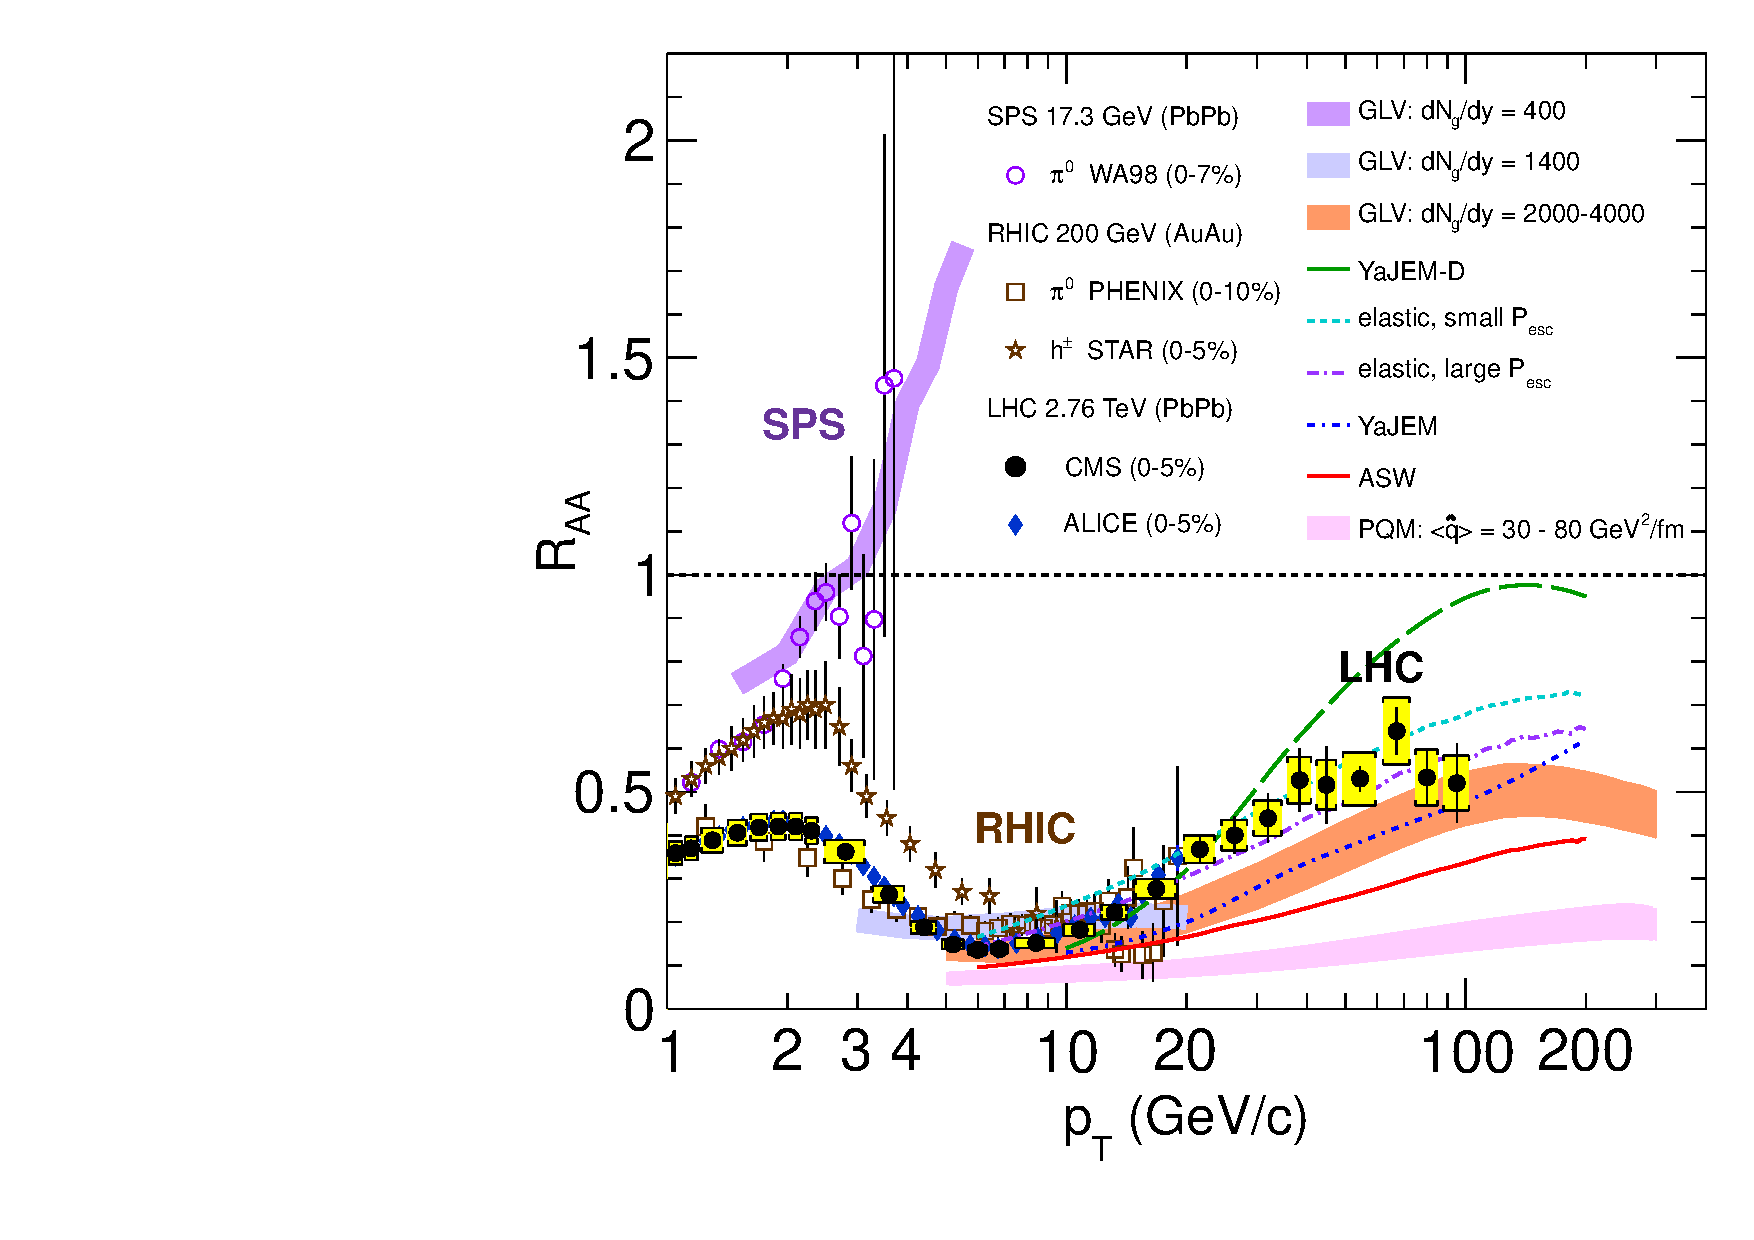
\includegraphics[width=0.5\textwidth]{ksfigures/CMSRAA.pdf}
\caption{Transverse momentum dependence of nuclear modification factor $R_{\rm AA}$ for charged particles produced in central heavy-ion collisions at LHC and lower energies. The curves and bands represent different model calculations. Reproduced from~\cite{CMS:2012aa}.}
\label{figks:CMSRAA}
\end{figure}

The CMS and ALICE experiments also measured the $R_{\rm AA}$ $p_{\rm T}$ dependence for different collision centralities~\cite{CMS:2012aa,Abelev:2012hxa}. The charged-particle production is, as expected, less and less suppressed as one moves from central to peripheral Pb--Pb collisons. The ATLAS collaboration reported similar results, presented as $R_{\rm CP}$ as a function of $p_{\rm T}$, where $R_{\rm CP}$ stands for a quantity analogue  to that defined in Eq.~\ref{eqks:RAA} using the normalized ratio of heavy-ion results at different centralities (the subscript CP indicates the central-to-peripheral ratio), commonly using the most peripheral class available for normalization.
%R_AA from CMS up to 100 GeV
\subsection{Identified-hadron spectra}
\label{subsecks:identspectra}
Study of the particle composition as a function of $p_{\rm T}$ reveals a mass hierarchy, interpreted as resulting from a common radial-velocity field created during the expansion of the dense-matter fireball. Such a collective flow arises in strongly interacting matter in the presence of a pressure gradient. Having the same velocity, heavier particles (e.g. protons) will acquire a larger momentum than lighter mesons. This effect is  visible in Fig.~\ref{figks:IdentPartSpec}, where the $p_{\rm T}$ spectra for pions, kaons, and protons measured by the ALICE experiment~\cite{Abelev:2012wca,Abelev:2013vea} exploiting various particle-identification techniques, are presented for the top 5\,\% central events, and compared to RHIC data~\cite{Adler:2003cb,Abelev:2008ab}. As the slope of the $p_{\rm T}$ spectra is affected by the particle masses ($m$), more instructive is to demonstrate it using the transverse-mass  ($m_{\rm T} = \sqrt{p_{\rm T}^2 + m^2}$) spectra, as done in~\cite{Heinz:2013th}. From the simultaneous blast-wave fit~\cite{Schnedermann:1993ws} to the $p_{\rm T}$ spectra (excluding pions with $p_{\rm T} < 0.5$~GeV and kaons with $p_{\rm T} < 0.35$~GeV where resonance decays largely contribute; more proper way would be to account for resonances and their decays in the fit, this is in preparation), the kinetic freeze-out temperature ($T_{\rm kin}$, temperature when the hadrons cease to interact) and an average radial velocity ($\langle \beta \rangle$) is estimated. The two parameters were extracted for different centralities, and they were found to be strongly correlated, since they both determine the slope of the $p_{\rm T}$ spectra. Both $T_{\rm kin}$ and $\langle \beta \rangle$ are higher compared to RHIC, and they depend on centrality: $T_{\rm kin}$ being lower for more central collisions, while $\langle \beta \rangle$ increases. The values reached for 5\,\% of most central collisions are $T_{\rm kin} \approx 95$~MeV and $\langle \beta \rangle \approx 0.65$, the latter being more than 10\,\% above the RHIC value~\cite{Adams:2005dq}. The blast-wave studies are being improved, sophisticating the model as mentioned above, exploiting data on other particle species, and using various assumptions about which particles have a common $T_{\rm kin}$ and which have a different one (i.e. accounting for differences in cross sections at low energies). Such studies will remain (useful) approximations of full hydrodynamical calculations coupled with a microscopic hadron-transport model.

The $p_{\rm T}$ spectra were compared further to various hydrodynamical-model calculations~\cite{Shen:2011eg,Bozek:2012qs,Werner:2012xh,Karpenko:2012yf}, and a fair description for the bulk production, up to transverse momenta 2--3~GeV, i.e. where such models are applicable, is observed for central collisions. In some cases~\cite{Karpenko:2012yf,Karpenko:2011qn} the agreement is improved by supplementing the hydrodynamical calculations with a hadronic rescattering code (UrQMD~\cite{Bass:1998ca}, in this occasion). The Krakow model~\cite{Bozek:2011ua,Bozek:2011gq} uses bulk viscosity corrections at freeze-out to describe deviation from equilibrium, which seems successful in reproducing the data. But going to more peripheral collisions the hydrodynamical description becomes worse at higher $p_{\rm T}$ and shows the limits of the hydrodynamical models. This could indicate the onset of a non-thermal (hard) component, which in more peripheral collisions is not dominated by the flow-boosted thermal component~\cite{Bozek:2012qs}.

\begin{figure}
\centering
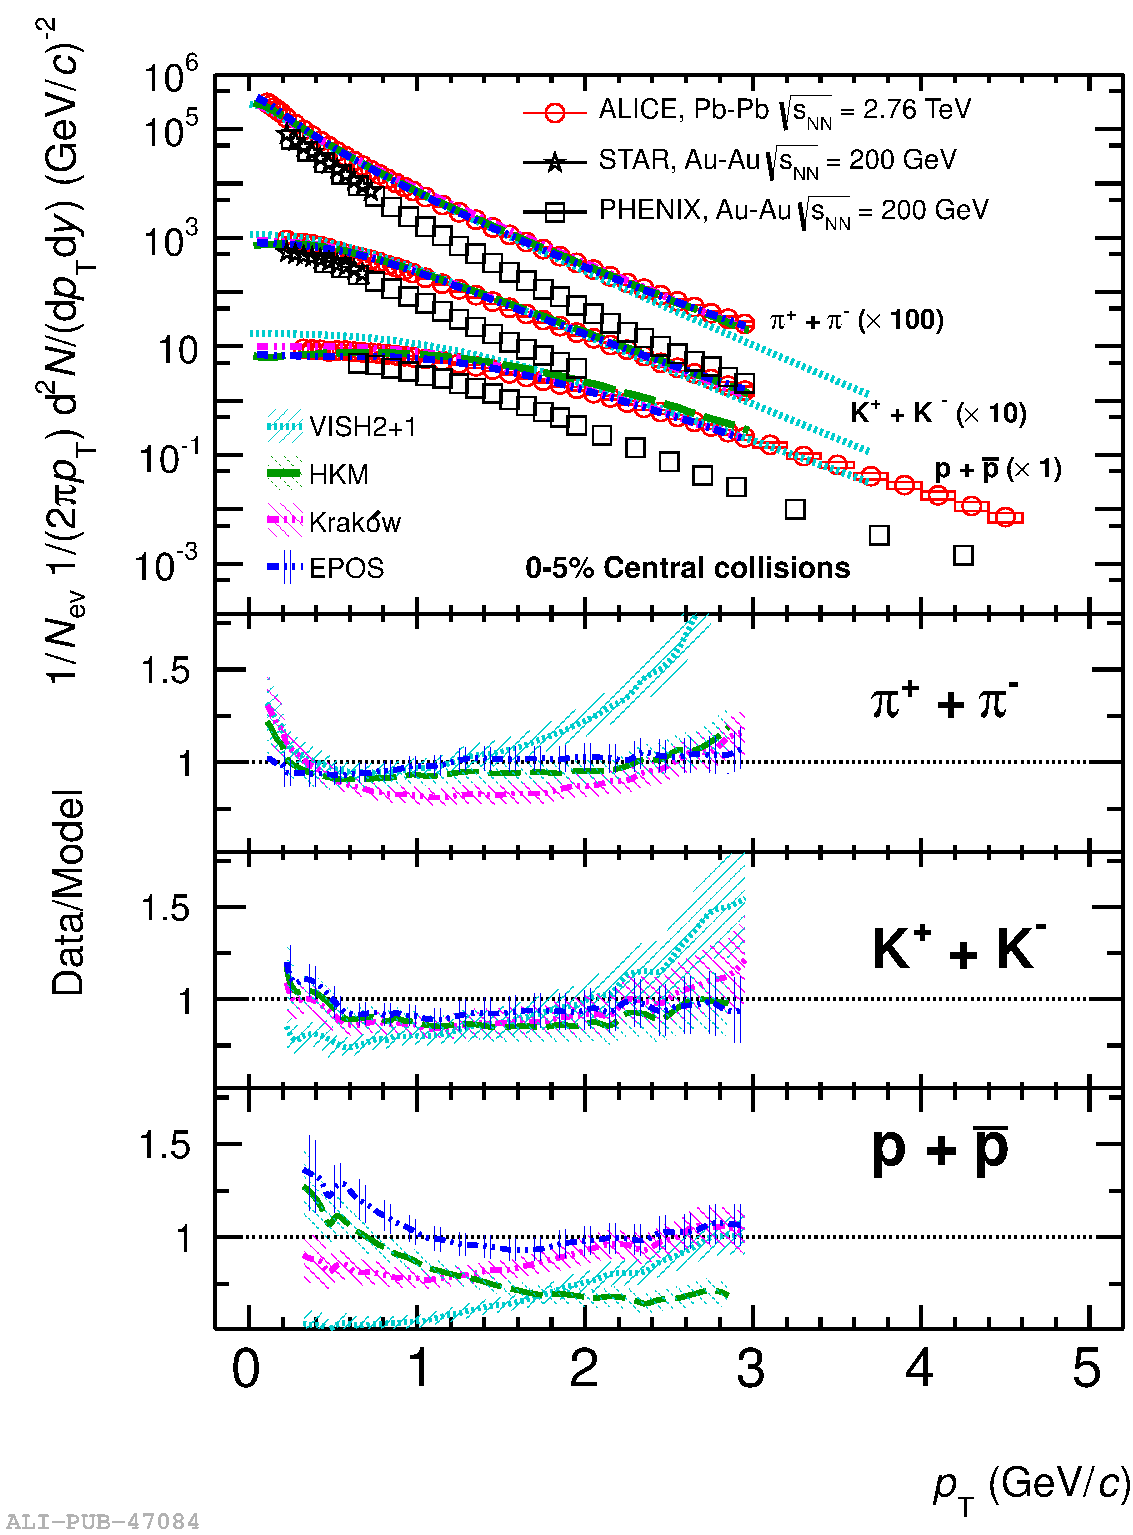
\includegraphics[width=0.5\textwidth]{ksfigures/IdentPartSpec.pdf}
\caption{Transverse momentum spectra for pions, kaons, and protons (sum of particles and antiparticles) produced in 5\,\% of most central Pb--Pb collisions at LHC, compared to the RHIC measurements and different model calculations. Adapted from~\cite{Abelev:2012wca}.}
\label{figks:IdentPartSpec}
\end{figure}

\begin{figure}
\centering
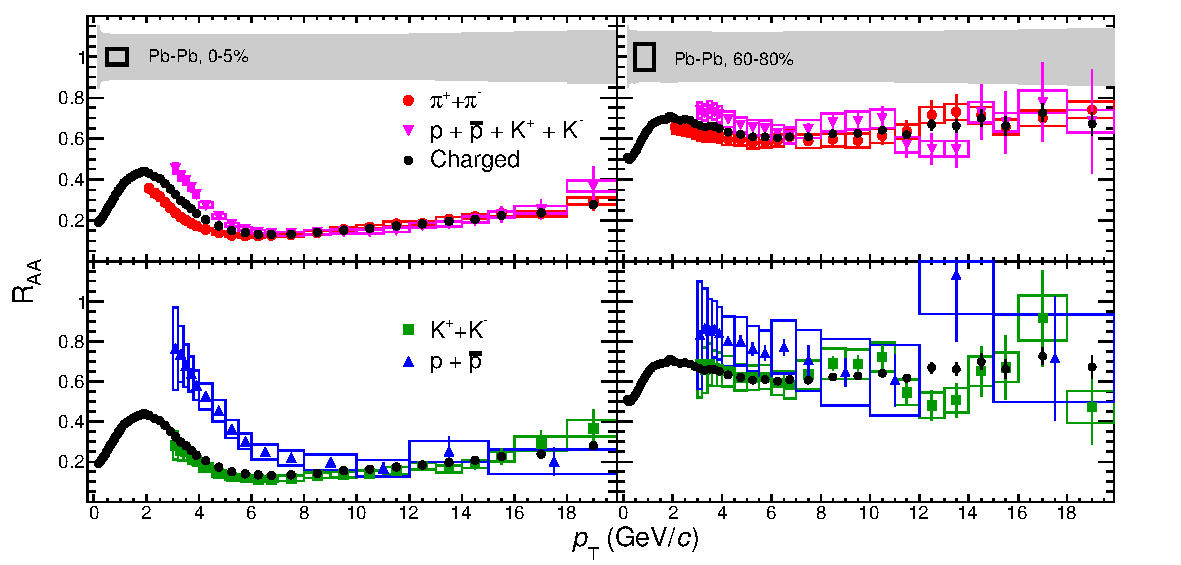
\includegraphics[width=0.75\textwidth]{ksfigures/IdentHighPtRAA.pdf}
\caption{Nuclear modification factor $R_{\rm AA}$ for pions, kaons, and protons (sum of particles and antiparticles), and averaged for charged particles, as a function of $p_{\rm T}$ for central (left, 0--5\,\%) and peripheral (right, 60--80\,\%) Pb--Pb collisions. Reproduced from~\cite{Abelev:2014laa}.}
\label{figks:IdentPartRAA}
\end{figure}

The $p_{\rm T}$ spectra of identified charged hadrons are determined up to $p_{\rm T} = 20$~GeV~\cite{Abelev:2014laa}, exploiting the measurement of ionization energy losses in the ALICE TPC in the relativistic rise region. Figure~\ref{figks:IdentPartRAA} presents these results normalized to the pp baseline, as $R_{\rm AA}$ for pions, kaons, and protons, compared to the (averaged) charged-particle data. It is clearly seen that for $p_{\rm T}$ above 7--8~GeV the behaviour for all particle species coincides. For lower $p_{\rm T}$ a mass hierarchy appears: the heavier the particle, the lower its suppression. These observations suggest the presence of three regions in transverse momentum:
\begin{itemize}
    \item{bulk region, low $p_{\rm T}$ up to 2--3~GeV, where the production comes from the hadronization of high-density strongly-interacting matter created in a heavy-ion collision, reflecting collective radial flow, fairly described (at least for central collisions) by hydrodynamical models;}
    \item{intermediate region, in $p_{\rm T}$ up to 7--8~GeV, where still a mass splitting among various particle species persists that can be attributed a reminiscence of radial flow (the difference has to disappear for $p_{\rm T}$ values significantly larger than particle masses), however, additional ideas were put forward to push further in $p_{\rm T}$ this mass distinction, such as constituent-quark recombination~\cite{Hwa:2006zq} which would favour baryons to acquire larger $p_{\rm T}$ than mesons;}
    \item{fragmentation region, above 7--8~GeV in $p_{\rm T}$, where the different hadron species exhibit a common suppression pattern, and consequently their relative abundances are the same as in pp collisions, naturally explained as being fragmentation products of a high-$p_{\rm T}$ parton coming from a hard scattering at early stage (which itself is quenched by the surrounding high-density matter).}
\end{itemize}

\begin{figure}
\centering
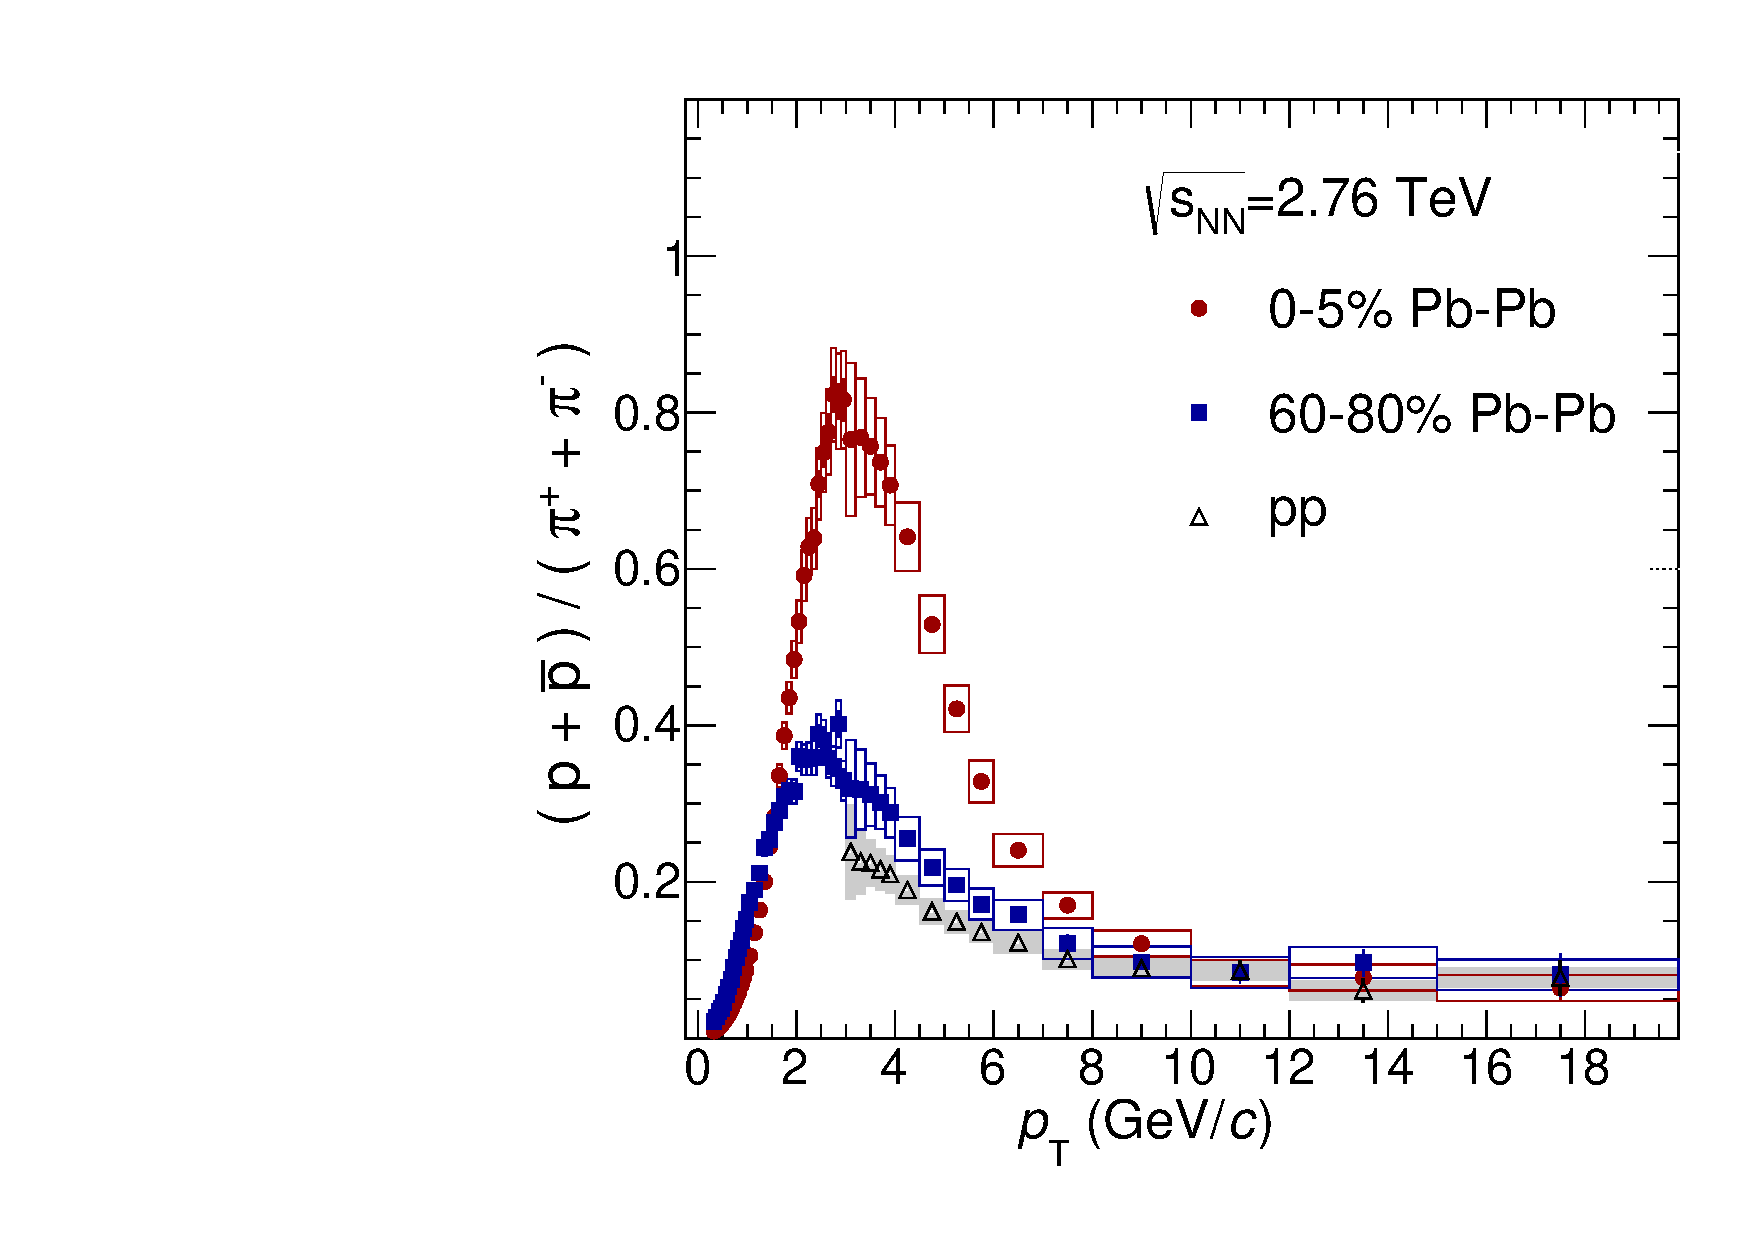
\includegraphics[width=0.5\textwidth]{ksfigures/ProtonToPion.pdf}
\caption{Ratio of proton-to-pion yields as a function of $p_{\rm T}$ measured in central (0--5\,\%) and in peripheral (60--80\,\%) Pb--Pb collisons, and in pp collisions. Reproduced from~\cite{Abelev:2014laa}.}
\label{figks:ProtonToPion}
\end{figure}

To look in detail into the intermediate region, it is instructive to plot the proton-to-pion ratio as a function of $p_{\rm T}$, Fig.~\ref{figks:ProtonToPion}. The striking effect is that for central collisions at $p_{\rm T}$ around 2.5--3~GeV this ratio is more than a factor three higher than the value for pp collisions. This so-called baryon anomaly was observed already at RHIC~\cite{Abelev:2006jr,Adare:2013esx}, and certainly the low-$p_{\rm T}$ rise is explained by the hydrodynamical radial flow. In the intermediate region, where the hydrodynamics ceases to work (at $p_{\rm T}$ around 2~GeV), still the hydrodynamic radial flow continues to affect the baryon-to-meson ratio towards higher $p_{\rm T}$, and the behaviour is qualitatively described by models involving constituent-quark recombination~\cite{Fries:2003kq} or baryon string-junction transfer along the axis of a fragmenting jet~\cite{Aurenche:2011rd}. These models, however, tend to predict an anomalous baryon-to-meson ratio even for significantly higher $p_{\rm T}$ than actually observed. On the other hand, a smooth connection between the hydro-described bulk region and the normal-ratio fragmentation region, using a realistic radial-flow profile, will probably move the border between the intermediate and fragmentation regions to lower than observed values. Therefore, a comprehensive description of the particle production in the intermediate region is still an open, and experiment driven issue. Recently, a good description has been obtained
by EPOS model~\cite{Werner:2012xh}, where the interaction between bulk matter (which thermalizes and flows) and jets is considered.

%Pion, Kaon, proton R_AA up to 20 GeV
%pi/p baryon anomaly
\subsection{Strange-particle production}
\label{subsecks:strangespectra}
Historically, the enhancement of strangeness production was among the first signatures proposed to signal a qualitatively different state of matter, expected to be created in ultra-relativistic heavy-ion collisions~\cite{Rafelski:1982pu,Koch:1986ud}. The strangeness increase in high-temperature QCD matter is motivated by two reasons: the relevant quark masses drop from their constituent to their bare values, and then the strange-quark mass becomes comparable to the temperature, consequently the production rates for different light quarks tend to equalize. Strangeness enhancement was already observed at lower energies, e.g. at the SPS~\cite{Margetis:2000sv,Andersen:1999ym,Antinori:2010jm,Alt:2008qm}, as well as at RHIC~\cite{Abelev:2007xp}. The systematic study of strangeness production at the LHC is under way in ALICE~\cite{ABELEV:2013zaa,Abelev:2013xaa}. In addition to charged kaons, the measurements include topologically identified particles (K$_{\rm s}^0$, $\Lambda$, $\Xi^-$, and $\Omega^-$), and resonances containing strangeness.

\begin{figure}
\centering
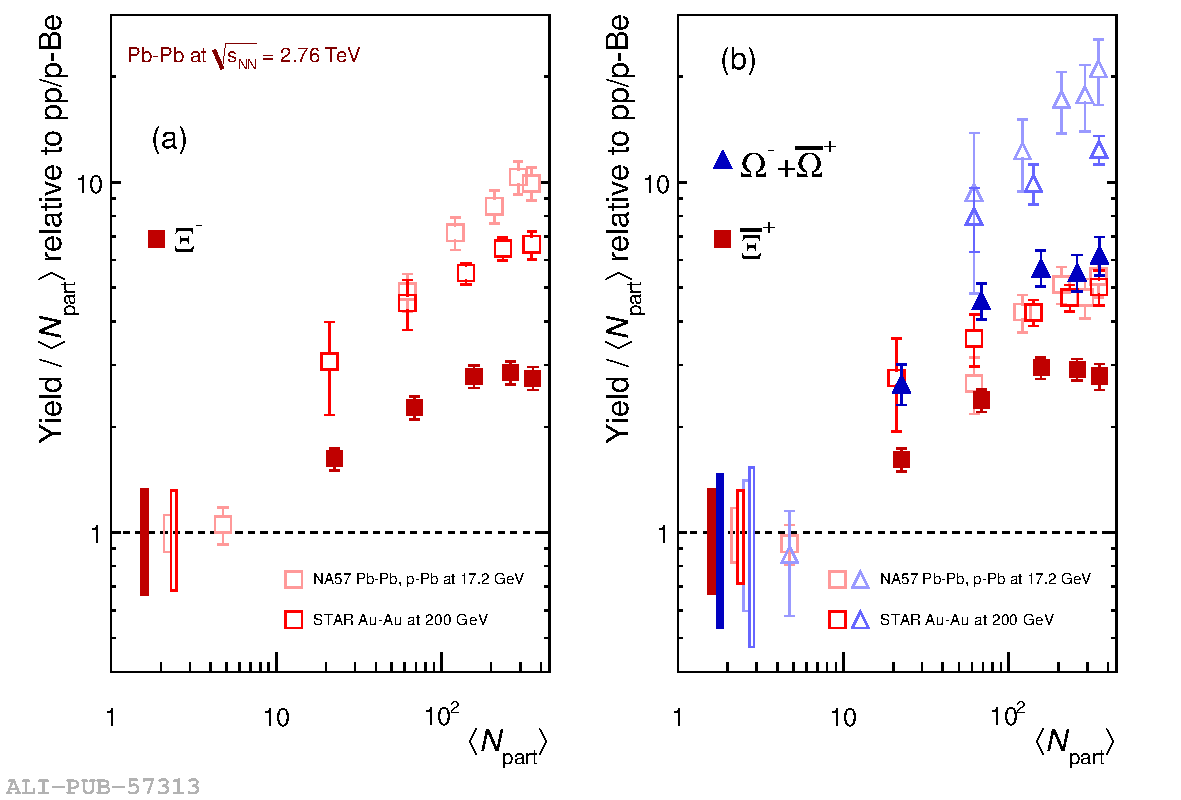
\includegraphics[width=0.75\textwidth]{ksfigures/StrangenessEnhancemet.pdf}
\caption{Strangeness enhancement for $\Xi$ and $\Omega$ at the LHC as the function of the mean number of participants, compared to the results obtained at CERN SPS and RHIC. Reproduced from~\cite{ABELEV:2013zaa}.}
\label{figks:StrangeEnhancement}
\end{figure}


The enhancement of strangeness production is confirmed at the LHC, see Fig.~\ref{figks:StrangeEnhancement}, albeit the enhancement factor, expressed as the ratio of the yield per participant in AA collisions to that in pp (or pA) collisions, decreases slowly with the collision energy. This reflects the fact that the production of strange particles per pion in heavy-ion collisions practically saturates as $\sqrt{s_{\rm NN}}$ reaches few tens of GeV (i.e. the top SPS energy), while in pp it still increases from RHIC to the LHC, and only at the highest energy ($\sqrt{s} = 7$~TeV) seems to cease its growth. However, these asymptotic yields per pion are significantly higher in heavy-ion collisions than in pp interactions, signaling the change of the mechanism of strangeness production. As predicted, to achieve such an increase, roughly a factor of two more strange quarks is necessary, compared the extrapolation from pp collisions. The strange-particle yields are well described by statistical hadronization models (Sec.~\ref{subsecks:yields}) without any strangeness suppression factor, needed in the case of pp and pA collisions.

The strange-particle $R_{\rm AA}$ is also influenced by strangeness enhancement, especially in the bulk and intermediate $p_{\rm T}$ regions~\cite{Knospe:2013tda}. As already mentioned, kaons, including K$_{\rm s}^0$, are above the pion curve. The strange baryons have larger $R_{\rm AA}$ than protons, and $R_{\rm AA}$ increases with the strangeness content, exceeding unity for $\Omega^-$. With increasing $p_{\rm T}$, the strangeness $R_{\rm AA}$ goes progressively closer to the common fragmentation behaviour for all other particle species, still being for $\Omega^-$ at $p_{\rm T} \approx 7$~GeV above the others. These measurements are at this point limited by the available statistics.

\begin{figure}
\centering
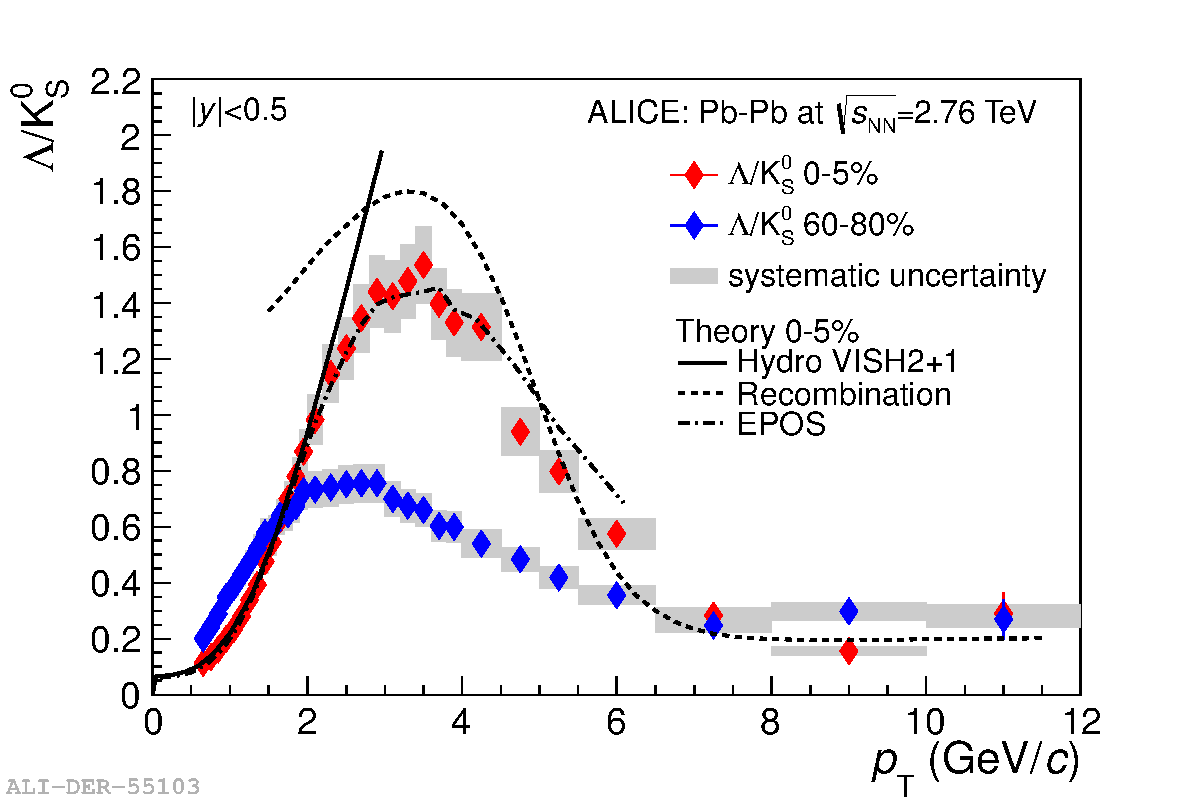
\includegraphics[width=0.5\textwidth]{ksfigures/LambdaToK0T.pdf}
\caption{Ratio of $\Lambda$-to-K$_{\rm s}^0$ yields as a function of $p_{\rm T}$ measured in central (0--5\,\%) and in peripheral (60--80\,\%) Pb--Pb collisons compared to model calculations. Reproduced from~\cite{Abelev:2013xaa}.}
\label{figks:LambdaToK}
\end{figure}


Baryon-to-meson ratio in the strangeness sector is very similar to that of proton-to-pion. The $\Lambda$-to-K$_{\rm s}^0$ ratio as a function of $p_{\rm T}$ is shown in Fig.~\ref{figks:LambdaToK} together with hydrodynamical- and recombination-model calculations~\cite{Song:2007ux,Song:2008si,Song:2011qa}. The EPOS model~\cite{Werner:2012sv}, which includes the hydrodynamical expansion and, at higher $p_{\rm T}$, the (mini-)jet fragmentation with an interaction between jets, describes the experimental measurement fairly well.
%K0, Lambda, Xi, Omega R_AA
%Lambda, Xi, Omega enhancements
%K0/Lambda
\subsection{Resonance and light-nuclei production}
\label{subsecks:resonace}
The resonances are interesting to study in heavy-ion collisions, because of their short lifetime they may decay inside the medium, before the kinetic freeze-out. If a decay product scatter changing its momentum, the parent resonance  cannot be observed by invariant-mass reconstruction, and that leads to an apparent depletion of the resonance yield, which is dependent on the resonance lifetime. On the other hand, resonances can be also recreated during the elastic scattering phase having a large cross-section for $s$-channel production at very low energies. Therefore, the comparison of the different-lifetime-resonance yields with hadronic-transport models gives valuable information about the time evolution during the late stage of heavy-ion collisions.

At the LHC, the ALICE collaboration reported the measurements of K$^*(892)^0$ and $\phi$ mesons~\cite{Abelev:2014uua}. The yield of K$^{*0}$ relative to other particles (e.g. K$^-$) decreases significantly for more central collisions, while the $\phi$ yield normalized in the same way is compatible with being independent of centrality. This is qualitatively understood by an order of magnitude different lifetimes for the two resonances (4.2~fm and 46~fm for K$^{*0}$ and $\phi$, respectively). A substantially lower production of K$^{*0}$ in central collisions also means that the regeneration is not effective enough to compensate the decay rate. Similar observations were made at RHIC~\cite{Aggarwal:2010mt}. The $\phi$ meson, being relatively long-lived to be treated as stable on the time scale of the heavy-ion collision, is of special interest. Its mass is close to that of the lightest baryons, therefore, the $\phi$ $p_{\rm T}$ spectrum can differentiate mass-dependent effects and constituent-quark-number effects. When compared to various hydrodynamical-model calculations~\cite{Shen:2011eg,Qiu:2011hf,Bozek:2012qs,Song:2012tv,Song:2013qma,Karpenko:2011qn,Karpenko:2012yf}, in general, the measured $\phi$ yields are overpredicted. In particular, the VISHNU model (VISH2+1 coupled to UrQMD)~\cite{Song:2012tv,Song:2013qma} is at lower $p_{\rm T}$ (below 1.5~GeV) by a factor of two above the data (probably due to an overestimated regeneration of $\phi$ in the hadronic phase), and fails to describe the shape of the $p_{\rm T}$ distribution. The Krakow model~\cite{Bozek:2012qs} and HKM (hydrokinetic model --- ideal hydrodynamic coupled to UrQMD)~\cite{Karpenko:2011qn,Karpenko:2012yf} are much closer to the data. The experimental results, presented in Fig.~\ref{figks:PhiTop}, indicate compatibility between proton and  $\phi$ $p_{\rm T}$ spectra up to 5~GeV in 10\,\% of most central Pb--Pb collisions, favouring thus the radial-flow explanation of the baryon anomaly to the constituent-quark-recombination one. At RHIC, from $\phi$ elliptic-flow and $p_{\rm T}$-spectrum measurements other conclusion was reached~\cite{Abelev:2007rw}. In peripheral collisions, the proton-to-$\phi$  ratio is not constant (see Fig.~\ref{figks:PhiTop}), possibly implying that the quark content may influence a particle-production mechanism.

\begin{figure}
\centering
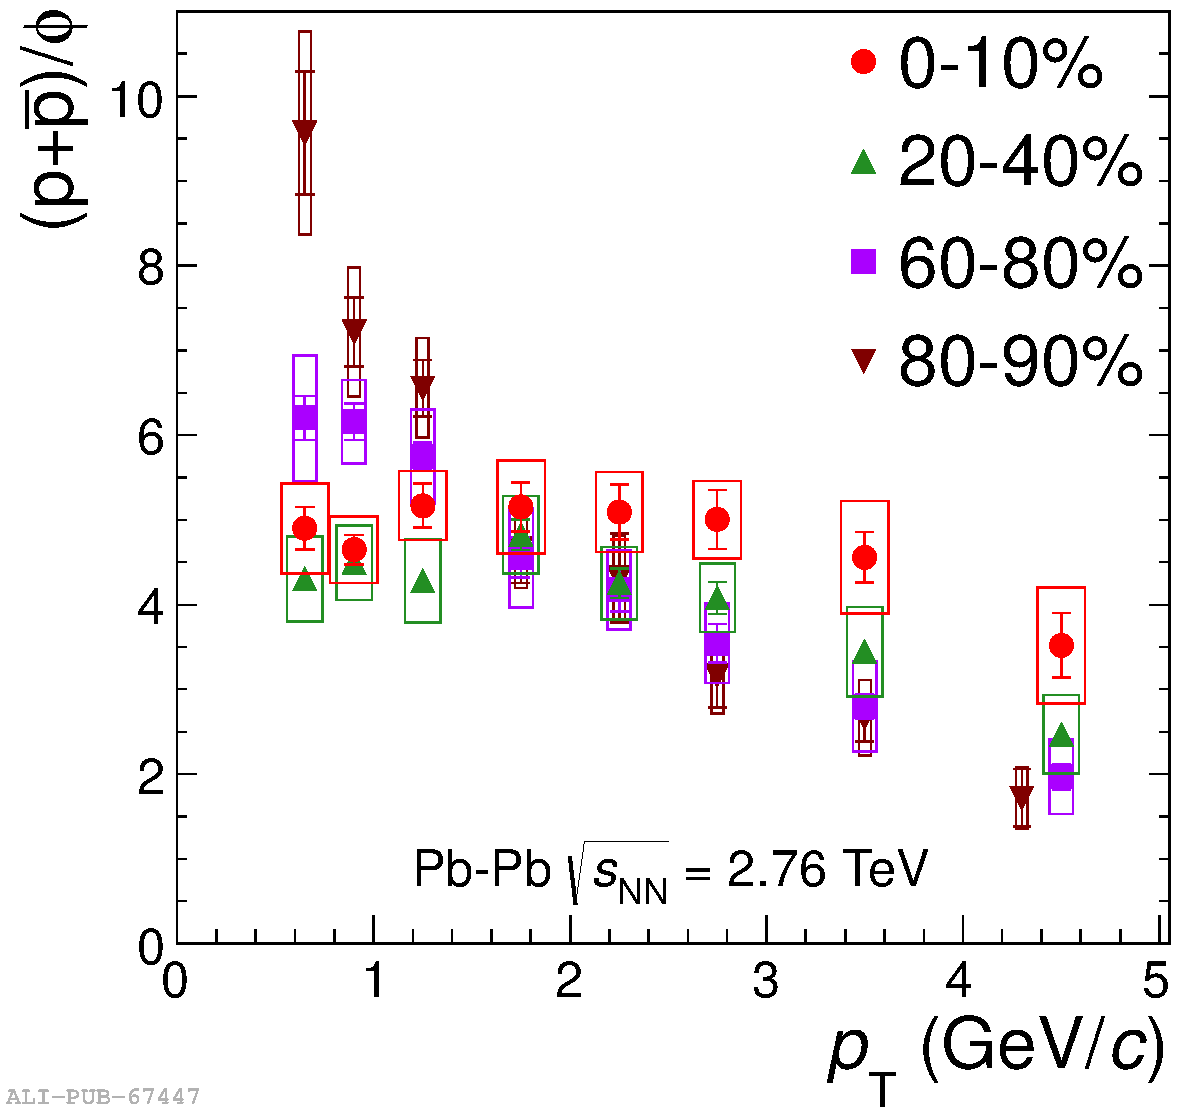
\includegraphics[width=0.5\textwidth]{ksfigures/ProtonToPhi.pdf}
\caption{Ratio of proton-to-$\phi$ yields as a function of $p_{\rm T}$ measured for four centrality intervals in Pb--Pb collisons. Reproduced from~\cite{Abelev:2014uua}.}
\label{figks:PhiTop}
\end{figure}

The high density of particles produced in heavy-ion collisions implies substantial rates for light-nucleus and hypernucleus production. The interest of such measurement is to study the production mechanism of such state, their coalescence coefficients, and their thermodynamical equilibrium with other particles. The light nuclei, such as d, t, $^3$He, and $^4$He, and corresponding antinuclei, were observed in heavy-ion collisions at RHIC and the LHC, and quantitative results for d and $^3$He were reported by ALICE. These measurements use the particle identification based on the specific ionization losses in TPC and the TOF measurement. The production of hypernuclei (nuclei containing one or more strange baryons) is of additional interest since the (unknown) properties of hypernuclei, their masses and decays, can be measured. The ALICE collaboration reconstructed the $^3_{\Lambda}{\rm H} \rightarrow ^3{\rm He} + \pi^-$ decays, as well as the charge-conjugated ones, opening the study in this field at the LHC, following the first antihypertriton measurement at RHIC~\cite{Abelev:2010rv}. Searches for more exotic states, such as the H-dibaryon ($\Lambda\overline{\Lambda}$ bound state or six-quark state), the $\overline{\Lambda}\overline{\rm n}$ bound state, and the $\Phi(1860)$ pentaquark have not given any positive signal.
%phi, deuteron, He3 He4
\subsection{Particle yields}
\label{subsecks:yields}
%particle yields vs thermal models
The particle yields at mid-rapidity are obtained by integration of the transverse-momentum spectra fitted to the blast-wave functional dependence (or other suitable function), in order to extrapolate below the lowest measured $p_{\rm T}$. Traditionally, the particle yields in heavy-ion collisions are studied within statistical hadronization models~\cite{Andronic:2008gu,Andronic:2011yq,Cleymans:1998fq,Becattini:2009fv}. These models are based on the grand-canonical ensemble, describing the system with the temperature ($T_{\rm ch}$), the baryon chemical potential ($\mu_{\rm b}$), and the volume in thermal and chemical equilibrium with the rest. Knowing these parameters it is straightforward to calculate the average number of various particles in the system. All the resonance and other unstable states, summed-up in the grand potential (usually with an upper mass cut-off about $2$~GeV, as above the resonance spectrum is not well known), are decayed into observed particles and compared to the measurements. The temperature $T_{\rm ch}$ is interpreted as the chemical freeze-out temperature, below which the energy of hadronic re-scattering is lower than the threshold for inelastic interactions, and thus the particle composition remains unchanged. The assumption of a chemical freeze-out temperature common to all particle species surmises that the particle composition in a heavy-ion collisions is fixed in a very narrow entropy-density window during the expansion of the high-density and high-temperature fireball.

The statistical models were used to describe the heavy-ion collision data from very low energies up to RHIC with a good agreement for most of the particle species. The temperature $T_{\rm ch}$ practically does not change with the collision energy, therefore, a reasonable estimate for LHC is the value observed at RHIC, $T_{\rm ch} = 164$~MeV; the chemical potential has to be very low as the ratio of particles to antiparticles is for all species compatible with unity; $\mu_{\rm b} = 1$~MeV is usually assumed. The predictions using these parameter values are compared in Fig.~\ref{figks:YieldProtonKaon} with the measurements of yield ratios: p$/\pi$ and K$/\pi$, for different centralities (expressed by particle density). The conclusion is that the measured proton yield for central Pb--Pb collisions at the LHC is by a factor of about 1.5 lower than predicted. In order to describe the proton measurement, significantly lower $T_{\rm ch}$ is needed (about 152~MeV), but then the yields of multi-strange baryons are underestimated. Trying to fit the temperature to the available data gives an estimate of $T_{\rm ch} \approx 156$~MeV, however, the fit description is not as good as it was at lower energies. Moreover, it is hard to expect that the chemical freeze-out temperature would decrease at higher energy.

\begin{figure}
\centering
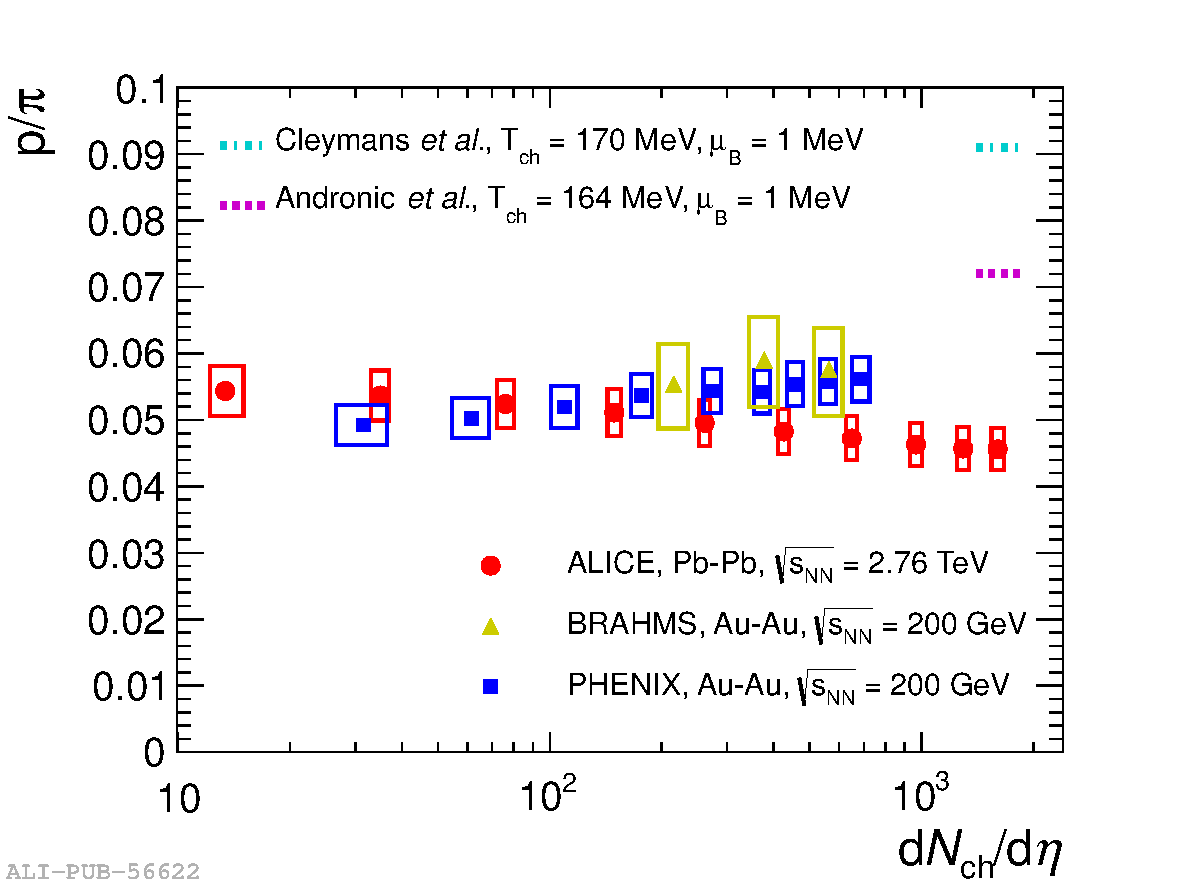
\includegraphics[width=0.4\textwidth]{ksfigures/YieldProtonToPion.pdf}
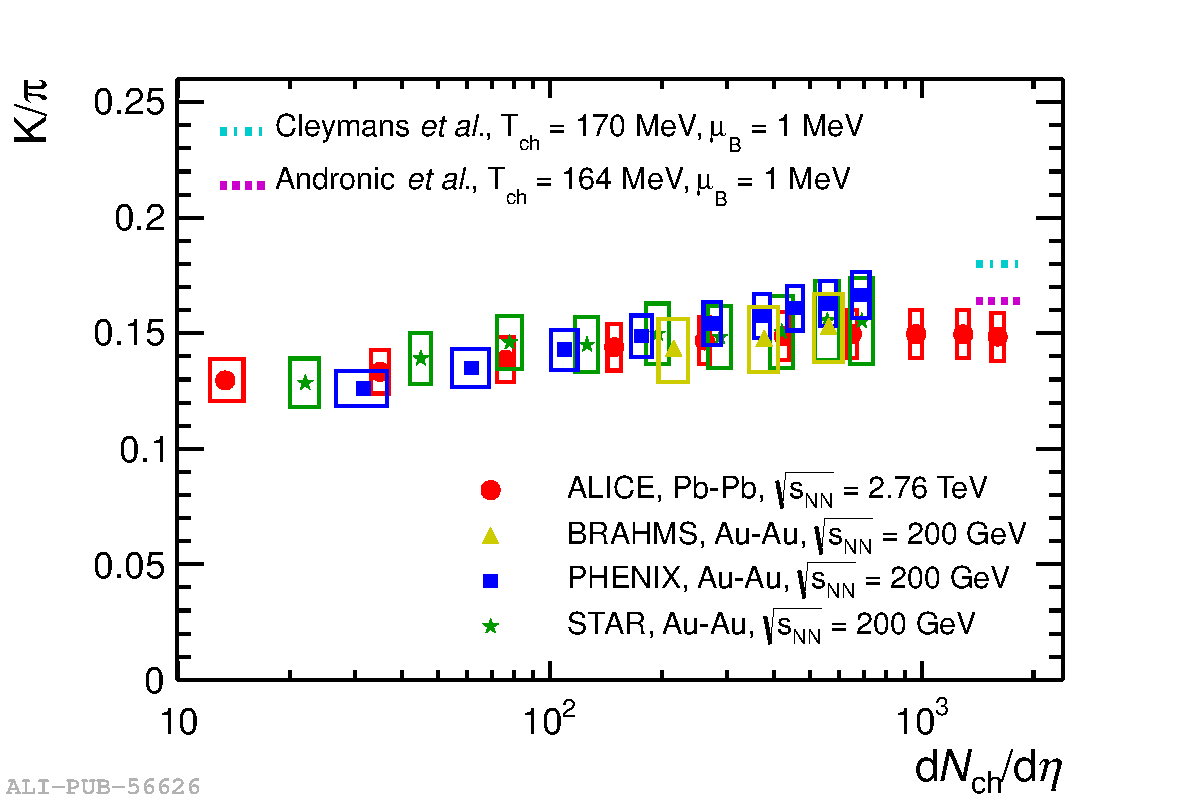
\includegraphics[width=0.4\textwidth]{ksfigures/YieldKaonToPion.pdf}
\caption{Ratios of proton-to-pion (left) and kaon-to-pion (right) yields at mid-rapidity as a function of charged-particle density in Pb--Pb collisons compared to the RHIC measurements~\cite{Abelev:2008ab,Bearden:2001qq,Adler:2003cb}. Reproduced from~\cite{Abelev:2013vea}.}
\label{figks:YieldProtonKaon}
\end{figure}


It seems that such problems were there partly already at RHIC. The discrepancy being smaller, and uncertainties in proton-yield corrections, lead to the fact that it was considered not significant. There are a few attempts to explain the lower proton yield at the LHC:
\begin{itemize}
\item{The baryons can annihilate in re-scattering with antibaryons, even after chemical freeze-out. This will affect protons more then strange baryons, because protons have larger density, and the annihilations with a strange partner are penalized due to presence of kaon(s) in final state, which shrink the phase space and thus lower the cross section of such cross-flavour annihilation. The effect was confirmed with UrQMD calculations~\cite{Karpenko:2012yf,Steinheimer:2012rd,Becattini:2012xb}, and the longer lifetime of the hadron gas makes it larger at the LHC than at RHIC. It was also shown that multi-meson interactions, recreating the baryon--antibaryon pairs, are not, at decreasing temperature, effective enough to compensate the loss~\cite{Pan:2012ne}.}
\item{The statistical hadronization model assumes strictly the same $T_{\rm ch}$ for all particles, which may not necessarily be true. Motivated by recent lattice QCD calculations, flavour- and mass-dependent prehadronic states in QGP may alter the effective phase-transition temperature resulting in an non-uniform freeze out~\cite{Ratti:2011au}. This will consequently modify the yields predicted by the model.}
\item{The high-mass resonances, not accounted for in the model, would presumably increase mostly the pion yield. Because of the number of these resonances can raise exponentially with the mass~\cite{Hagedorn:1965st,RHagedorn:1968}, even their production being exponentially damped, the effect may be non-negligible. This would lower the p$/\pi$ model prediction~\cite{Andronic:2008gu}, however, in a similar way at the LHC and at RHIC.}
\item{The statistical hadronization model can be modified, incorporating non-equilibrium effects. In fact the model was used also to describe particle yields in pp, and even in e$^+$e$^-$, interactions, however, an additional parameter suppressing strangeness production had to be used. Introducing two parameters regulating the population of phase space, separately for light-quarks and strange quark, allows for good description of the experimental measurements.~\cite{Rafelski:2010cw,Petran:2013lja}}
\end{itemize}
The lower-than-expected proton yield observed at the LHC was one of the first surprises from the heavy-ion programme, and its origin has yet to be established.

%... not sign for a large experimental discrepancy between RHIC and the LHC...
